\documentclass[../../thesis.tex]{subfiles}

\newcommand{\norm}[1]{\left\lVert#1\right\rVert}

\begin{document}


%%%%%%%%%%%%%%%%%%%%%%%%%%%%%%%%%%%%%%%%%%%%%%%%%%%%
%\begin{abstract}                          % Abstract of not more than 200 words.
%Cyber-physical systems are found in many applications such as power networks, manufacturing processes, and air and ground transportation systems. Maintaining security of these systems under cyber attacks is an important and challenging task, since these attacks can be erratic and thus difficult to model. Secure estimation problems study how to estimate the true system states when  measurements are corrupted and/or control inputs are compromised by attackers. The authors in \cite{Fawzi:2014} proposed a secure estimation method when the set of attacked sensors (sensors, controllers) is fixed. In this chapter, we extend these results to scenarios in which the set of attacked sensors can change over time. We formulate this secure estimation problem into the classical error correction problem \cite{tao11} and we show that accurate estimation can be guaranteed. Furthermore, we propose a combined secure estimation method with our proposed secure estimator and the Kalman Filter for improved practical performance. Finally,  we demonstrate the performance of our method through simulations of two scenarios where an unmanned aerial vehicle is under attack.
%\end{abstract}

In this chapter, we develop a secure estimator for a general linear system and demonstrate its effectiveness through an example of an unmanned aerial vehicle (UAV) under cyber attack.
In the next chapter, we extend these results to two classes of nonlinear systems and apply the secure estimator to the nonlinear power system.

Cyber-physical systems (CPSs) are found in many applications such as power networks, manufacturing processes, air and ground transportation systems. They consist of physical components such as actuators, sensors and controllers that communicate with each other over a network \cite{kim2012cyber}. 
For example, UAVs may obtain position measurements from a GPS or communicate with a remote control center (RCC). Although communication networks are often protected by security measures, cyber attacks can still take place when a malicious attacker obtains unauthorized access, launching jamming attacks \cite{Gligor}, or spoofing sensor readings and sending erroneous control signals to actuators \cite{Mo}. For CPS, cyber attacks not only compromise information but can also cause damage in the physical process, ranging from power systems \cite{teixeira2010cyber, liu2011false} to UAVs \cite{Hu:2016uav}. This presents new challenges and thus demands new strategies and algorithms \cite{Sastry}.

Maintaining security of these systems under cyber attacks is an important and challenging task, since these attacks can be erratic and thus difficult to model. Secure estimation problems study how to estimate the true system states when  measurements are corrupted and/or control inputs are compromised by attackers. 
In designing such estimators, it is desirable to make as few assumptions about the attackers as possible. This is because it is very difficult, if not impossible, to predict the behavior of attackers, and when an attack signal violates the assumptions of a secure estimator, then this estimator would fail to detect the attack.
\cite{Fawzi:2014} proposed a novel secure estimation method assuming that attack signals can be arbitrary and unbounded. However, one limitation of their proposed estimator is that the set of attacked sensors (sensors, controllers) is assumed to be fixed. 
In this chapter, we extend these results to scenarios in which the set of attacked sensors can change over time. We formulate this secure estimation problem into the classical error correction problem \cite{tao11} and we show that accurate estimation can be guaranteed. Furthermore, we propose a combined secure estimation method with our proposed secure estimator and the Kalman Filter (KF) for improved practical performance. Finally,  we demonstrate the performance of our method through simulations of two scenarios where a UAV is under cyber attack.
\\
\\
\noindent
\textit{This chapter is an adaptation of the paper in \cite{Hu:2016uav}.}

\section{Introduction}
%%%%%%%%%%%%%%%%%%%%%%%%%%%%%%%%%%%%%%%%%%%%%%%%%%%%

Researchers have studied various approaches to securing CPS. Each of them relies on specific assumptions about attackers' strategies and it is rarely the case, if not impossible, that one estimator/detector can protect against all possible attacks. 
For example, \cite{Tong, KwonACC, liu2011false, teixeira2010cyber} studied optimal attack strategies for different control systems and applications. 
From the controller's point of view, \cite{Bullo, Liu} assumed that the attack signal would follow certain probabilistic distributions and then designed filters to detect these attacks.
In \cite{Wu, Basar, Basar2, Walrand, Pappas}, the authors used the game theory framework, where the controller and attacker are players with competing goals in a game. 
Attackers are assumed to adopt specific strategies that maximize a certain cost and the controller or estimator is designed to minimize such a cost.
Finally, the authors of \cite{KwonCDC} proposed a hybrid controller, where each constituent controller protects the system against a specific type of attack.

More recently,  \textit{Fawzi et al.} studied secure estimation of a discrete time linear time invariant (LTI) system and proposed in \cite{Fawzi:2014} a secure estimation method for arbitrary attacks. 
%\cite{chong2016characterising} proposed the security index of a discrete time LTI system under sensor attacks as a quantitative measure on the security of an observable system.
Later, \cite{Pajic:2014} and \cite{shoukry2016smt} extended this work by relaxing the assumption of having an exact system model and proposed an Satisfiability Modulo Theory (SMT)-based observer that handles large systems with thousands of sensors. 
One limiting assumption of \cite{Fawzi:2014}, \cite{Pajic:2014} and \cite{shoukry2016smt} is that the set of attacked sensors is fixed and can not change over time. 
Therefore, if a malicious attacker is aware of this assumption, then she can exploit this weakness and attack different sensors at different time steps so that such an estimator would fail to detect the presence of the attack.

In this chapter, we focus on sensor attacks on CPS and attempt to design a secure estimator for LTI systems based on as few assumptions about the attacker as possible. 
First, we do not assume that the attack signals follow any stochastic distributions, and thus our proposed estimator works for arbitrary and unbounded attacks.
Second, we allow the set of attacked sensors to change over time.
The only assumption we make is that the number of attacked sensors is sparse.
%are interested in the case in which the set of attacked sensors can change over time. 
%By doing so, our proposed estimator can protect the system against more general attack scenarios than that presented in \cite{Fawzi:2014}. 
%We believe this is a significant contribution, because it is difficult, if not impossible, to anticipate cyber attackers' strategies and behavior, thus an estimator that is able to handle more general attacks is an improvement. 
Such attacks are found in many practical situations, and can be launched in both the cyber and the physical domain.
For example, security studies on the current traffic infrastructure \cite{ghena2014traffic} demonstrated that once a cyber attacker gains access to the traffic network at a single point, the attacker can send commands to any traffic intersection in the network. 
In other words, the attacker can freely attack a different set of traffic signals (sensors) at any time. Indeed, an attacker who desires to travel through a set of roads as fast as possible would attack different traffic lights to always give herself green lights as she moves through the road network. 
%Also, even with physical attacks, there are practical examples where time-varying attacks are desirable. 
\cite{liu2014coordinated} describes a physical attack on a power system where a changing set of attacked sensors is desirable: in particular, the authors designed a multi-switch attack, in which different switches in a power network are attacked at different times, in order to lead to stealthy and wide-scale cascading failures in the power system.


We formulate this secure estimation problem into the classical error correction problem, from which we propose an $l_1$-optimization based estimator that is computationally efficient.
In addition, we prove the maximum number of sensor attacks that can be corrected with our estimator and propose to use pole placement techniques to design a feedback controller such that the resulting secure estimator can guarantee accurate estimation.
Finally, to improve the estimator's practical performance, we propose to combine our secure estimator with a KF, where the KF serves to filter out both occasional estimation attacks by the secure estimator and noisy measurements, and we demonstrate the effectiveness of the combined estimator using two examples of UAVs under adversarial cyber attacks.


%There are four main contributions in this chapter:
%First, we propose a secure estimator for an LTI system under sensor attacks, where the attacked sensors can change over time, and attack signals can be unbounded and arbitrary.
%The proposed estimator is based on $l_1$ optimization and is computationally efficient.
%Second, we prove the maximum number of sensor attacks that can be corrected with our estimator, which turns out to be the same as that of the estimator proposed in \cite{Fawzi:2014} with the mere requirement of a longer time window. In other words, compared to \cite{Fawzi:2014}, our estimator can protect the system against more general attacks, and at the same time, it does not compromise the number of attacks that can be corrected.
%Third, we propose to use pole placement techniques to design a feedback controller such that the resulting secure estimator can guarantee accurate estimation.
%Finally, we propose to combine our estimator with a KF to improve its practical performance, where the KF serves to filter out both occasional estimation attacks by the secure estimator and noisy measurements.



This chapter is organized as follows. A review of compressed sensing and error correction in given in Section \ref{sec:overview}, followed by Section \ref{sec:SE} which proposes a secure state estimator for an LTI system under sensor attack where the attacked sensors can change over time. 
Then, Section \ref{sec:design} describes how pole-placement can be used to design a good secure estimator and how it can be combined with a KF to improve its practical performance. 
Finally we demonstrate the performance of the combined secure estimator through two numerical examples of UAVs subject to adversarial attacks in Section \ref{sec:examples}. 


%\subsection{Notation}
%\begin{itemize}
%\item 
%$\lvert \textsf{supp} (x) \rvert $  denotes the support of vector $x$, i.e., the number of nonzero components in $x$\footnote{If $f$ is any real-valued or vector-valued function on a topological space $X$, the support of $f$, denoted by $\textsf{supp}(f)$, is the closure of the set points where $f$ is nonzero: $\textsf{supp}(f)  = \{ x \in X \,|\, f(x) \neq 0 \}$.}. 
%%\item 
%%$\norm{ x}_{l_1}:= \sum_{i=1} ^n \lvert x_i \rvert $ where $x \in \mathbb{R}^n$. Note that this is not the same as $\lvert \textsf{rowsupp} ( \cdot )  \rvert $ defined in \cite{Fawzi:2014}. 
%\item  
%For a matrix $M \in \mathbb{R}^{m \times n}$, $\mathcal{N} (M) = \{ x \in \mathbb{R}^n \lvert M x = 0 \}$ represents the null space of $M$. $\mathcal{R}(M)$ denotes the range space of $M$, and is defined as the set of all possible linear combinations of its column vectors.
%\end{itemize}



%%%%%%%%%%%%%%%%%%%%%%%%%%%%%%%%%%%%%%%%%%%%%%%%%%%%
%%%%%%%%%%%%%%%%%%%%%%%%%%%%%%%%%%%%%%%%%%%%%%%%%%%%
%%%%%%%%%%%%%%%%%%%%%%%%%%%%%%%%%%%%%%%%%%%%%%%%%%%%


\section{Review of Classical Error Correction}\label{sec:overview}
\subsection{Compressed Sensing}
Sparse solutions $x\in \mathbb{R}^n$, are sought to the following problem:
\begin{equation}
	\min_x \norm{x}_0 \text{ subject to } b= Ax
	\label{eq:CS}
\end{equation}
where $b \in \mathbb{R}^m$ are the measurements, and $A \in \mathbb{R}^{m\times n}~ (m \ll n)$ is a sensing matrix. $\norm{x}_0$ denotes the number of nonzero elements of $x$. The following lemma provides a sufficient condition for a unique solution to (\ref{eq:CS}).

\begin{lem} (\hspace{1sp}\cite{David_Chang}) \label{lem:CS}
If the sparsest solution to (\ref{eq:CS}) has $\norm{x}_0 = q$ and $m\ge 2q$ and all subsets of $2q$ columns of $A$ are full rank, then the solution is unique.
\end{lem}

\textit{Proof}:
Suppose the solution is not unique. Therefore, there exists $x_1 \neq  x_2$ such that $Ax _1 = b$ and $Ax_2 = b$ where $\norm{x_1}_0 = \norm{x_2}_0 = q$. Then, $A(x_1 - x_2) = 0$ and $x_1 - x_2 \neq 0$. Since $\norm{x_1-x_2}_0 \leq 2q$ and all $2q$ columns of $A$ are full rank (i.e., linearly independent), it is impossible to have $x_1-x_2\neq 0$ that satisfies $A(x_1-x_2) = 0$. This contradicts the assumption.
\hfill$\blacksquare$


\begin{remark}
(Measurement Noise) In practice, the measurements are noisy so one cannot assume that the $Ax$ term in (\ref{eq:CS}) is known with arbitrary precision. More appropriately, we need to assume that one is given noisy measurements, i.e., $b = Ax + \epsilon$, where $\epsilon$ represents measurement noise. In \cite{Candes_Tao}, the authors prove that one can recover approximately sparse signals with an error at most proportional to the noise level. 
An alternative is to combine secure estimation with a KF to improve the secure estimator's performance for noisy measurements as we propose later in this chapter: the KF filters out both occasional estimation errors by the secure estimator and noisy measurements.
\end{remark}

%%%%%%%%%%%%%%%%%%%%%%%%%%%%%%%%

\subsection{The Error Correction Problem \cite{tao11}}
Consider the classical error correction problem: $y=Cx + e$ where $C\in \mathbb{R}^{l\times n}$ is a coding matrix $(l > n)$ and assumed to be full rank. We wish to recover the input vector $x \in \mathbb{R}^n$ from corrupted measurements $y$. Here, $e$ is an arbitrary and unknown sparse error vector. To reconstruct $x$, note that it is obviously sufficient to reconstruct the vector $e$ since knowledge of $Cx + e$ together with $e$ gives $Cx$, and consequently $x$ since $C$ has full rank \cite{tao11}. In \cite{tao11}, the authors construct a matrix $F$ which annihilates $C$ on the left, i.e.,  $FCx = 0$ for all $x$. Then, they apply $F$ to the output $y$ and obtain
\begin{equation}
	\tilde y = F (Cx + e) = Fe.
\end{equation}
Thus, the decoding problem can be reduced to that of reconstructing a sparse vector $e$ from the observations $\tilde y = Fe$. Therefore, by Lemma \ref{lem:CS}, if all subsets of $2q$ columns of $F$ are full rank, then we can reconstruct any $e$ such that $\| e \|_0 \leq q$.





%%%%%%%%%%%%%%%%%%%%%%%%%%%%%%%%%%%%%%%%%%%%%%%%%%%%
%%%%%%%%%%%%%%%%%%%%%%%%%%%%%%%%%%%%%%%%%%%%%%%%%%%%
%%%%%%%%%%%%%%%%%%%%%%%%%%%%%%%%%%%%%%%%%%%%%%%%%%%%



\section{Secure Estimation}\label{sec:SE}

\subsection{Problem Formulation}
Consider the LTI system as follows:
\begin{equation}
\begin{aligned}
x(k+1) &= A_o x(k) + B u(k) \\
y(k) &= C x(k) + e(k),
\end{aligned} 
\label{eq:system_model_se}
\end{equation} 
where $x(k) \in \mathbb{R}^n$, $y(k) \in \mathbb{R}^p$ and $u(k) \in \mathbb{R}^m$ are the states, measurements and control inputs at time step $k$. $e(k) \in \mathbb{R}^p$ represents the attack signal at time $k$. Our goal is to reconstruct the initial state $x(0)$ of the plant from the corrupted observations $y(k)$'s where $k=0,...,T-1$.

The attack vector $e(k)$ is such that if the $i$-th sensor is attacked at time $k$, then $e_i(k)$, the $i$-th element of $e(k)$ is nonzero, otherwise $e_i(k) = 0$. We assume that the attack signal can be arbitrary and unbounded. In addition, we assume that the set of attacked sensors can change over time. As illustrated by the following example, if two sensors are attacked at each time step, we can have sensors 1 and 3 attacked at time step 0, sensors 2 and 3 attacked at time 1, and so on:
\begin{equation}
	\begin{bmatrix} e(0)  & \lvert & e(1) & \lvert &  ...  & \end{bmatrix} 
	= \begin{bmatrix} * & 0 & * & \cdots \\
					       0 & * & 0 & \cdots \\
					       * & * & 0 & \cdots \\
					       0 & 0 & * &\cdots 
			\end{bmatrix}, \nonumber \\
\end{equation}
where $*$ denotes a nonzero component (i.e., an attack or corruption). 

Furthermore, assume that a local control loop implements secure state feedback and is not subject to attack: $u(k) = Gx(k)$. 
This represents the following practical scenario: a physical system possesses a local control loop that has direct access to the state of the plant and can control the evolution of the physical system. 
This is reasonable if the sensors are connected to the local controller through a wired link that is not subject to external attacks. 
Also, as part of the overall plant, a higher-level supervisory and monitoring system receives measurements from the sensors through wireless and vulnerable communication links that are subject to attacks \cite{Fawzi:2014}. 
A concrete example is a UAV that uses measurements from onboard, hardwired sensors such as an Inertial Measurement Unit (IMU) for autopilot and trajectory following (i.e., secure local control loop), and communicates wirelessly with a remote control center (i.e., vulnerable link subject to attacks).
%In the case of UAVs, this corresponds to using measurements from onboard, hardwired sensors such as Inertial Measurement Units (IMU) for autopilot and trajectory following. 
The resulting closed loop system is:
\begin{equation}
\begin{aligned}
x(k+1) &= A x(k)\\
y(k) &= C x(k) + e(k),
\end{aligned} 
\label{eq:system_model_cl}
\end{equation} 
where the closed loop system matrix $A=A_o+BG$. 



Finally, we define the number of correctable attacks as follows:
\begin{definition}\label{def:num_err_change}
When the set of attacked sensors/nodes can change over time, $q$ errors are correctable after $T$ steps by the estimator/decoder $\mathcal{D}: {(\mathbb{R} ^p) } ^T  \rightarrow \mathbb{R}^n$ if for any $x(0) \in \mathbb{R}^n$ and any sequence of vectors $e(0),...,e(T-1)$ in $\mathbb{R}^p$ such that $\lvert \textsf{supp}(e(k)) \rvert \leq q$\footnote{$\lvert \textsf{supp} (x) \rvert $  denotes the support of vector $x$, i.e., the number of nonzero components in $x$. If $f$ is any real-valued or vector-valued function on a topological space $X$, the support of $f$, denoted by $\textsf{supp}(f)$, is the closure of the set points where $f$ is nonzero: $\textsf{supp}(f)  = \{ x \in X \,|\, f(x) \neq 0 \}$.}, 
we have $\mathcal{D} (y(0),...,y(T-1)) = x(0)$ where $y(k) = CA^k x(0) + e(k)$ for $k=0,...,T-1$.
\end{definition}


%%%%%%%%%%%%%%%%%%%%%%%%%%%%%%%%%%%%

\subsection{Methodology}

Let $E_{q,T}$ denote the set of error vectors $\begin{bmatrix} e(0); ~ ...~  ;  e(T-1) \end{bmatrix}   \in  \mathbb{R}^{p\cdot T} $ where each $e(k)$ satisfies $\|e(k)\|_0 \leq q \leq p$. 
\begin{eqnarray} \label{eq:sys_err_corr}
\begin{aligned}
	Y &\triangleq \begin{bmatrix} y(0) \\ y(1) \\ \vdots \\ y(T-1) \end{bmatrix}  = \begin{bmatrix} Cx(0) + e(0)\\ CA x(0) + e(1) \\ \vdots \\ CA^{T-1} x(0) + e(T-1) \end{bmatrix} \\
		& =
		\begin{bmatrix} C \\ CA \\ \vdots \\ CA^{T-1} \end{bmatrix} x(0) + E_{q,T}  \triangleq \Phi x(0) + E_{q,T}
		\label{eq:decoder_Phi}
\end{aligned}
\end{eqnarray}
where $Y \in \mathbb{R}^{p\cdot T}$ is a collection of corrupted measurements over $T$ time steps and $\Phi \in \mathbb{R}^{p\cdot T \times n}$ represents an observability-like matrix of the system. 
Here, we need to assume that $\operatorname{rank}(\Phi) = n$; otherwise, the system is unobservable and we cannot determine $x(0)$ even if there is no attack (i.e., $E_{q,T} = 0$).


Inspired by the error correction techniques proposed in \cite{tao11} and \cite{David_Chang}, we first determine the error vector $E_{q,T}$, and then solve for $x(0)$. 
Consider the $QR$ decomposition of $\Phi \in \mathbb{R}^{p\cdot T \times n}$,
\begin{eqnarray}
	\Phi = \begin{bmatrix} Q_1 & Q_2 \end{bmatrix} \begin{bmatrix} R_1 \\ 0 \end{bmatrix} = Q_1 R_1
\end{eqnarray}
where $\begin{bmatrix} Q_1 & Q_2 \end{bmatrix} \in \mathbb{R}^{p\cdot T \times p\cdot T}$ is orthogonal, $Q_1 \in \mathbb{R}^{p\cdot T\times n}, Q_2 \in \mathbb{R}^{p\cdot T \times (p\cdot T-n)}$, and $R_1 \in \mathbb{R}^{n\times n}$ is a rank-$n$ upper triangular matrix.
Pre-multiplying (\ref{eq:decoder_Phi}) by $\begin{bmatrix} Q_1 & Q_2 \end{bmatrix} ^\top$ gives:
\begin{equation}
	\begin{bmatrix} Q_1 ^\top \\ Q_2 ^\top \end{bmatrix} Y = \begin{bmatrix}R_1 \\ 0  \end{bmatrix} x(0) + \begin{bmatrix} Q_1 ^\top \\ Q_2^\top \end{bmatrix} E_{q,T}.
	\label{eq:QR}
\end{equation}
We can compute $E_{q,T}$ by using the second block row:
\begin{equation}
	\tilde Y \triangleq Q_2^\top Y = Q_2^\top E_{q,T}
	\label{eq:E_est}
\end{equation}
where $Q_2^\top \in \mathbb {R} ^{ (p\cdot T-n) \times p\cdot T}$.
From Lemma \ref{lem:CS}, (\ref{eq:E_est}) has a unique, $s$-sparse solution (where $s\le q\cdot T$) if all subsets of $2s$ columns (at most $2 q\cdot T$ columns) of $Q_2^\top$ are full rank. Clearly, this is a reasonable assumption if $(p\cdot T-n) \ge 2q\cdot T$. Therefore, we consider solving the following $l_1$-minimization problem:
\begin{equation}
	\hat{E}_{q,T} = \arg \min_E \norm { E}_{l_1} \text{ s.t. } \tilde Y = Q_2^\top E,
	\label{eq:solve_E}
\end{equation}
where $\norm{E}_{l_1}:= \sum_{i=1} ^{p\cdot T} \lvert E_i \rvert$. Now, given the vector $\hat{E}_{q,T}$, we can compute $x(0)$ from the first block row of (\ref{eq:QR}) as follows:
\begin{equation}
	x(0) = R_1^{-1} Q_1^\top (Y- \hat{E}_{q,T})
	\label{eq:QR1}
\end{equation}
The following lemma provides the conditions under which the solution to (\ref{eq:QR1}) exists and is unique.

\begin{lem} \label{lem:EC}
	$x(0) $ is the unique solution if $\lvert \textsf{supp}( \Phi z) \rvert > 2 s = 2 (q\cdot T)$ for all $z \in \mathbb{R}^n \backslash \{ 0 \}$.
\end{lem}

\textit{Proof}:
We first prove the claim C1: if $\lvert \textsf{supp}( \Phi z) \rvert > 2 s = 2 (q\cdot T)$ for all $z \in \mathbb{R}^n \backslash \{ 0 \}$ then all subsets of $2s$ columns of $Q_2^\top$ are full rank. Then by Lemma \ref{lem:CS} and noting that by definition the null space of $Q_2^\top$ equals the column space of $\Phi$, we have $x(0) $ is the unique solution.

Proof of C1 by contradiction: Suppose there exist $2s$ columns of $Q_2^\top$ that are linearly dependent. Then, there exists $E_0 \neq 0$ such that $Q_2^\top E_0 = 0$ where $\lvert \textsf{supp}(E_0) \rvert \le 2s$. Since the null space of $Q_2^\top$ equals the column space of $\Phi$, there exists $z$ such that $E_0 = \Phi z$ (i.e., $E_0$ is in the column space of $\Phi$). Then, $ \lvert  \textsf{supp}(\Phi z) \rvert = \lvert \textsf {supp} (E_0) \rvert \le 2s $ (contradiction).
\hfill$\blacksquare$\\

The sufficient condition, provided in Lemma \ref{lem:EC}, for the existence of a unique solution to (\ref{eq:QR1}) is hard to check as it requires satisfiability of the condition for all $z \in \mathbb{R}^n \backslash \{ 0 \}$. In the following Theorem, we prove an equivalent, yet simple-to-check, sufficient condition that only needs to be verified for the eigenvectors of $A$.



\begin{theorem}\label{thm:SE} 
Let $A \in \mathbb{R}^{n\times n}, C \in \mathbb{R}^{p\times n}$. Assume that $C$ is full rank, $(A,C)$ is observable and $A$ has $n$ distinct positive eigenvalues such that $0 < \lambda_1 < \lambda_2 < \cdots < \lambda_n$. 
Define:
\begin{itemize}
\item
$s_i \triangleq \lvert \textsf{supp} (Cv_i) \vert$, where $v_i$ is an eigenvector of $A$, 
\item
$\mathcal{S} \triangleq \{ s_1, s_2, \cdots, s_n \}$,
\item
For every $m \in \{2, \ldots, n\}$, let $\mathcal{S}_m$ be any subset of $\mathcal{S}$ with $m$ elements, define $T_{\mathcal{S}_m} \triangleq \frac {  (m-2) \cdot p + \min \mathcal{S}_m } {\max \mathcal{S}_m - 2q }$.
Then $T_m$ is chosen such that $T_m > T_{\mathcal{S}_m}$ for all subsets $\mathcal{S}_m$, i.e., all subsets of $m$ elements from the set $\mathcal{S}$.
\end{itemize}

Choose $T$ such that  $T \ge \max \{ T_2, \cdots, T_n \}$.
Then, the following are equivalent:

\begin{equation}
\begin{aligned} 
 (i)  &~\forall v_i \in \mathbb{R}^n \text{ where } Av_i =\lambda_i v_i, ~ \lvert \textsf{supp}(Cv_i) \rvert > 2q  \\
  (ii)  &~\forall v_i \in \mathbb{R}^n \text{ where } Av_i =\lambda_i v_i,  ~\lvert \textsf{supp} (\Phi v_i) \rvert > 2q \cdot T  \\
  (iii) &~  \forall z \in \mathbb{R}^n\backslash \{0 \}, \lvert \textsf{supp} (\Phi z) \rvert > 2 q \cdot T  \nonumber %~~~~~~~~ \text{(i.e. condition (ii) in Equation (\ref{eq:connection}))} \nonumber 
\label{eq:new_condition}
\end{aligned}
\end{equation}
\end{theorem}

\textit{Proof}:
Interested readers are referred to proof for Theorem \ref{thm:SE} in our archived paper \cite{Chang:2017}.
\hfill$\blacksquare$\\

Theorem \ref{thm:SE} states that if the feedback system and the secure estimator are designed such that all the conditions in the theorem are satisfied, then our proposed secure estimator can guarantee accurate correction of $q$ errors by checking the following very simple condition:
\begin{equation}\label{eq:distinct}
\forall v_i \in \mathbb{R}^n \text{ where } Av_i =\lambda_i v_i, ~ \lvert \textsf{supp}(Cv_i) \rvert > 2q.  %\nonumber
\end{equation}


%%%%%%%%%%%%%%%%%%%%%%%%%%%%%%
%\subsubsection{Proof of Theorem \ref{thm:SE} \cite{Chang:2017}} 
%In order to prove Theorem 1, we make use of Lemma \ref{lem:two_vec} and Proposition \ref{prop:m_vec} (see Appendix).
%
%First, it is simple to prove that $(i)$ and $(ii)$ are equivalent: $\lvert \textsf{supp} (\Phi v_i) \rvert = \sum_{k=0}^{T-1} \lvert \textsf{supp} (CA^k v_i ) \rvert = \sum_{k=0}^{T-1} \lvert  \textsf{supp} (\lambda_i^k C v_i )\rvert  = T\cdot  \lvert \textsf{supp} (C v_i) \rvert  $. 
%
%Second, we want to show that $(ii)$ and $(iii)$ are equivalent. The direction $(iii) \implies (ii)$ is trivial, since $(ii)$ is a specific case of (iii) with $z = v_i$. The other direction is more complex. Note that $A$ is diagonalizable, therefore its eigenvectors form a basis for $\mathbb{R}^n$. Now consider the decomposition of $z $ in the eigenbasis of $A$, i.e. $z = \sum_{i=1}^n \alpha_i v_i$ with $\alpha_i \neq 0$ for at least one $i$. 
%\begin{enumerate}
%\item $m=1$: Suppose there exists $z \in \mathbb{R}^n \backslash \{ 0\}$ such that $ \lvert \textsf{supp} (\Phi z) \rvert \le 2 q \cdot T$. Without loss of generality, let $\alpha_i \neq 0$ and $\alpha_j= 0$ for all $j \neq i$, then, $2 q \cdot T \ge \lvert \textsf{supp} (\Phi z) \rvert = \lvert \textsf{supp} (\alpha_i \Phi v_i) \rvert = \lvert \textsf{supp} (\Phi v_i) \rvert $ for all $T$ (contradiction, $\because \forall v_i, \lvert \textsf{supp} (\Phi v_i) \rvert  > 2 q \cdot T$). 
%%\item $m=2$: By Lemma \ref{lem:two_vec}, if we choose $T>T_2$.
%\item $m\ge 2$: By Lemma \ref{lem:two_vec} and Proposition \ref{prop:m_vec}, if we choose $T>T_m$ for each value of $m$, respectively.
%\end{enumerate}
%We need to choose $T$ to satisfy the worst case for any $m$ such that $n \ge m \ge 2$. Thus, if $T \ge \max \{ T_2, \cdots, T_n \}$, then $(ii)$ and $(iii)$ are also equivalent. Note that $T_m$ is chosen to satisfy $T_m > T_{\mathcal{S}_m}$ for all subsets $\mathcal{S}_m$, i.e., $T_m = \max_{\mathcal{S}_m}( T_{\mathcal{S}_m})+1$.
%\hfill$\blacksquare$\\






%%%%%%%%%%%%%%%%%%%%%%%%%%%%%%%%%%%%%%

\subsection{Number of Correctable Errors}\label{sec:max_q}

Given that the set of attacked nodes can change over time and $e(k)$ satisfies $\lvert \textsf{supp} (e(k)) \rvert \le q$ for all $k$, we prove in Proposition \ref{prop:maximum} (see below) that the maximum number of correctable errors (as defined in Definition \ref{def:num_err_change}) by our decoder is $\lceil p/2-1 \rceil$, where $p$ is the number of measurements. 

\begin{proposition}\label{prop:maximum} 
Let $A_0 \in \mathbb{R}^{n \times n}$, $B \in \mathbb{R}^{n \times m}$ and $C \in \mathbb{R}^{p \times n}$ and assume that the pair ($A_0$, $B$) is controllable, $C$ is full rank and each row of $C$ is not identically zero. Then there exists a finite set $F \subset \mathbb{R}_+$ such that for any choice of $n$ numbers $\lambda_1, \cdots, \lambda_n \in \mathbb{R}_+ \backslash F$ such that $0<\lambda_1< \cdots < \lambda_n$, there exists $G \in \mathbb{R}^{m \times n}$ such that:
\begin{itemize}
\item
The eigenvalues of the closed-loop matrix $A~(= A_0+BG)$ are $\lambda_1, \cdots, \lambda_n$.
\item
If the pair ($A, C$) is observable, then the number of correctable errors for the pair ($A, C$) is maximal after $T= \max\{n, T^*\}$ time steps and is equal to $\lceil p/2-1 \rceil$, where $T^*$ is the value of $T$ from Theorem \ref{thm:SE}. 
\end{itemize}
\end{proposition}

\textit{Proof}:
The proof for Proposition 4 in \cite{Fawzi:2014} shows that if the chosen poles $\lambda_1, \cdots, \lambda_n$ are distinct, positive and do not fall in some finite set $F$, then there is a choice of $G$ such that the eigenvalues of $A~(=A_0+B)$ are exactly $\lambda_1, \cdots, \lambda_n$, and the corresponding eigenvectors $v_i$ are such that $\lvert \textsf{supp} (C v_i) \rvert = p$. Thus, by Theorem 1, the number of correctable errors for $(A,C)$ is $\lceil p/2-1 \rceil$.
\hfill$\blacksquare$\\

In addition, recall that $E_{q,T}$ consists of the error vectors $e(0), \cdots, e(T-1)$ stacked vertically and our proofs for the existence of a unique solution to (\ref{eq:QR1}) are independent of how the individual error (nonzero) terms are distributed in the vector $E_{q,T}$. Thus, we can remove the assumption: $\lvert \textsf{supp} (e(k)) \rvert \le q$ for all $k$, and allow $e(k)$ to appear in an arbitrary fashion, e.g. $\lvert \textsf{supp} (e(0)) \rvert = 2q$ and $\lvert \textsf{supp} (e(1)) \rvert = 0$, as long as $\sum_{k=0}^{T-1} \lvert \textsf{supp} (e(k)) \rvert \leq q\cdot T$, then our $q$-error-correcting estimator can still recover the true states. In other words, our proposed secure estimator can protect the system against more general attacks where the number of attacked sensors is not necessarily less than or equal to $q$ at every time step.


%%%%%%%%%%%%%%%%%%%%%%%%%%%%%%%%%%%%%%%%%%%%%%%%%%%%
%%%%%%%%%%%%%%%%%%%%%%%%%%%%%%%%%%%%%%%%%%%%%%%%%%%%
%%%%%%%%%%%%%%%%%%%%%%%%%%%%%%%%%%%%%%%%%%%%%%%%%%%%


\section{Estimator Design}\label{sec:design}
%%%%%%%%%%%%%%%%%%%%%%%%%%%%%%%%%%%%%%%%%%%%%%%%%%%%%%%

In the classical error correction problem, to ensure accurate estimation, the coding matrix must satisfy the Restricted Isometry Properties (RIP) conditions  \cite{tao11}, which are extremely difficult to check in general. In practice, Theorem \ref{thm:SE}.4 from\cite{tao11} is almost always used to design a coding matrix {\it a priori}. This theorem states that a coding matrix whose entries are sampled from independent and identical distributions satisfies the RIP condition with overwhelming probability. 
In secure estimation, however, it is impossible to choose such a coding matrix {\it a priori} because it is the observability matrix $\Phi$, which is structurally constrained: as shown in (\ref{eq:decoder_Phi}), $\Phi$ consists of $CA^{k}$'s where $k=\{0, \cdots, T-1\}$. In this Section, we use Condition \ref{eq:distinct} from Theorem \ref{thm:SE}, the results from Proposition 4 in \cite{Fawzi:2014} and state feedback to design a matrix $\Phi$ for accurate estimation. 


%%%%%%%%%%%%%%%%%%%%%%%%%%%%%%%%%%%%%%%%%%%%%%%%%%%%%%
%%%%%%%%%%%%%%%%%%%%%%%%%%%%%%%%%%%%%%%%%%%%%%%%%%%%%%


\subsection{System and Estimator Design}\label{sec:decoder_design}

Since conditions $(i)$ and $(iii)$ in Theorem \ref{thm:SE} are equivalent, condition $(i)$ can be used to design a state feedback controller such that the closed system can achieve accurate estimation. Therefore, given a controllable open-loop pair $(A_0,B)$, design $C$ and choose an adequate feedback control law $u(k) = G x(k)$ and construct a secure estimator such that:

\begin{enumerate}
	\item Each row of $C$ is not identically zero, and $C$ is full rank;
	\item The closed-loop matrix $A~(=A_0+BG)$ has $n$ distinct positive eigenvalues: $0< \lambda_1 < \lambda_2 < \cdots < \lambda _n$;
	\item $(A,C)$ is observable;
	\item The length of the sliding window of measurements $T$ of the estimator satisfies Theorem \ref{thm:SE}\footnote{We found that much smaller $T$'s are often sufficient for good secure estimation performance, i.e., to perfectly recover the attack signals. In all simulations in this chapter, $T=n$ is used, where $n$ is the number of states.};
	\item Maximize $q$ subject to: $\forall v_i \in \mathbb{R}^n$ where $Av_i = \lambda v_i$, $\lvert \textsf{supp} (C v_i)  \rvert > 2q$.
\end{enumerate}
Without loss of generality, the first condition holds. For example, if there exists a zero row in $C$, we can simply remove that row from $C$ without changing the system's behavior. Conditions 2, 3 and 4 are required for equivalence in Theorem \ref{thm:SE}. The last condition is needed for accurate estimation and for maximizing the number of correctable attacks. From Proposition \ref{prop:maximum} the maximum number of correctable attacks can be achieved when $\lvert \textsf{supp} (C v_i)  \rvert = p$ (i.e., the number of measurements) for all eigenvectors of $A$. 

Conditions 2, 3 and 5 depend on the feedback controller. So how do we choose a controller that achieves good performance in both control and secure estimation? Below, we describe an approach that we have taken in all simulations in this chapter, and has proved to work well. This is by no means the only method. First, we design a controller that achieves good control, for example, Linear Quadratic Regulators (LQR), which are optimal with respect to a certain quadratic cost function. However, these controllers may not have good secure estimation properties, meaning the value of $q$ that satisfies $\lvert \textsf{supp} (C v_i) \rvert > q$ for all eigenvectors of $A$ may be small, i.e., the resulting estimator can only correct few attacks. It is often easy to increase the value of $q$ and make the estimator more resilient to attacks by slightly perturbing the closed-loop poles from those resulting from the LQR controller, such as placing the poles closer to the origin, and making the poles more spread out amongst themselves. We chose to keep the perturbations small as to not lose too much control performance.  
Although this is a heuristic method, it is relatively easy to carry out in order to satisfy the above conditions; whereas in the classical error correction method \cite{tao11}, checking whether a coding matrix satisfies RIP is extremely difficult.

To summarize, we start from some optimal controller which may not result in a good estimator, then we perturb the closed-loop poles slightly to improve the resulting estimator's secure estimation capability. Therefore there is a trade-off between a system's control and secure estimation performances, and the feedback controller can be designed to achieve a desired trade-off between them.

%%%%%%%%%%%%%%%%%%%

\subsection{Combination of Secure Estimation and Kalman Filter}\label{sec:estimation}
Consider the state estimation problem for the following LTI system under attack:
\begin{equation}
\begin{aligned}
x(k+1) & = A x(k) + B u(k)\\
y(k) & = C x(k) + e(k) + v(k),
\end{aligned}
\end{equation}
where $x$, $y$, $u$ and $e$ are as defined in (\ref{eq:system_model_se}); and $v$ is a zero mean independent and identically distributed (i.i.d.) Gaussian measurement noise. 


\begin{figure}
\center
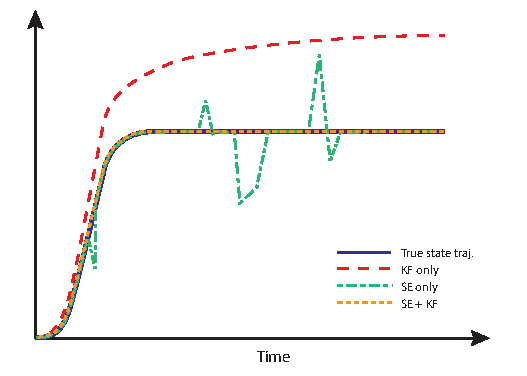
\includegraphics[width=0.6\textwidth]{chapters/se_linear/figures/qh/est_illu.pdf}
\caption{Illustrative comparison of three schemes: KF only (KF), secure estimator only (SE), secure estimator with a KF (SE+KF). KF fails to estimate the true state as attack signal is non-Gaussian. SE correctly estimates the system state most of the time but has occasional large estimation attacks. SE+KF tracks the true state trajectory perfectly.}
\label{fig:estimation}
\end{figure}


A KF can be used to estimate the states by modeling the attack signal as noise. More specifically, define a new measurement noise $\bar{v}(k) = e(k) + v(k)$ to give a new measurement equation $y(k) = C x(k) + \bar{v}(k)$. A KF can then estimate the states from the inputs $u(k)$ and the corrupted measurements $y(k)$ \cite{KwonACC}. 
One caveat with this method is that KFs assume zero mean and i.i.d. white Gaussian measurement noise, however, attack signals are usually erratic and may be poorly modeled by Gaussian processes \cite{KwonACC}, i.e., $e(k)$ and consequently, $\bar v(k)$ may not be Gaussian. Take GPS spoofing attacks for example, attack signals are often structured to resemble normal GPS signals or can be genuine GPS signals captured elsewhere.  
When the system is subjected to attacks that are poorly modeled by Gaussian processes, it is reasonable to expect KFs to fail to recover the true states. 
Figure \ref{fig:estimation} gives an illustrative example where an attack signal that increases linearly with time is injected into the measurements of state $x_i$. The red dashed line shows a plausible estimated state trajectory from a KF.

On the other hand, our proposed secure estimator does not assume the attack signal to follow any model, and therefore, it works for arbitrary and unbounded attacks. 
The only assumption is that the number of attacked sensors is sparse, i.e., less than $\lceil p/2-1\rceil$. 
As the set of attacked sensors becomes less sparse, our secure estimator occasionally fails to recover the true states.
The green dashed line in Figure \ref{fig:estimation} depicts a possible result from this estimator: the estimated state trajectory follows the true trajectory most of the time with occasional attacks. 
%When we consider the system model (\ref{eq:noise_model}), i.e., taking into account the zero mean i.i.d. Gaussian process noise and measurement noise, we can relax the equality constraint ($\tilde Y = Q_2 ^\top E)$ as follows: $\min_E \norm{E}_{l_1}$ subject to $\norm { \tilde Y - Q_2^\top E}\le \epsilon$, where $\epsilon$ represents the amount of noise. Consequently, the secure estimator acts as a prefilter for the KF (for example, identifying erratic and large error) so that $\tilde v(k)$ is close to a zero mean i.i.d. Gaussian process even when the true attack signal $e(k)$ is not.
Based on these observations, we propose to combine our secure estimator with a KF to improve its practical performance, as detailed in Algorithm 1.
\begin{algorithm}
\caption{Combined secure estimator with KF}
\label{al:se_kf}
\begin{algorithmic}[1]
\State Initialize the KF
\For{each $k$}
	\If{$k \geq T$}
		\State Estimate the attack signal at time $k$, $\hat e(k)$, using secure estimator
	\Else
		\State Set $\hat e(k) = 0$
	\EndIf
	\State Form a new measurement equation: $\tilde y(k) =  C x(k) + \tilde v(k)$, where $\tilde y(k) = y(k) - \hat e(k)$ and $ \tilde v(k) = e (k) - \hat e(k) + v(k)$
	\State Apply standard KF using $u$ and $\tilde y$ 
\EndFor
\end{algorithmic}
\end{algorithm}


The intuition is that the secure estimator acts as a pre-filter for the KF, so that $\tilde v(k)$ is close to a zero mean i.i.d. Gaussian process even when the true attack signal $e(k)$ is not. 
More specifically, the secure estimator usually perfectly recovers $e(k)$, thus $e(k) - \hat e(k) = 0$ and $\tilde v(k) = v(k)$. 
What happens when the secure estimator fails? 
Equation \eqref{eq:sys_err_corr} shows that the estimated state at time $k$, $\hat x(k)$, does not directly depend on the estimated state at another time point $\hat x(\tau)$ ($t \neq \tau$).
As a result, when the secure estimator fails, its estimation error, $e(k) - \hat e(k)$, appears to be quite random. 
Putting these together: $\tilde v(k) = e(k) - \hat e(k) + v(k)$ is closer to a zero mean i.i.d. white Gaussian process than $\bar v(k)$ (i.e., the corresponding measurement noise if a KF is applied directly to estimate the states), which improves the KF's performance.
Finally, the \textit{if} statement in Algorithm 1 ensures that the secure estimator always has access to $T$ past measurements, as required by Theorem \ref{thm:SE}.

Next, we demonstrate the effectiveness of our proposed method through simulations of a UAV under two types of adversarial attacks, which also provides a realistic example illustrating the behaviors described in this section.



%%%%%%%%%%%%%%%%%%%%%%%%%%%%%%%%%%%%%%%%%%%%%%%%%%%%
%%%%%%%%%%%%%%%%%%%%%%%%%%%%%%%%%%%%%%%%%%%%%%%%%%%%
%%%%%%%%%%%%%%%%%%%%%%%%%%%%%%%%%%%%%%%%%%%%%%%%%%%%
%%%%%%%%%%%%%%%%%%%%%%%%%%%%%%%%%%%%%%%%%%%%%%%%%%%%
%%%%%%%%%%%%%%%%%%%%%%%%%%%%%%%%%%%%%%%%%%%%%%%%%%%%
%%%%%%%%%%%%%%%%%%%%%%%%%%%%%%%%%%%%%%%%%%%%%%%%%%%%
%%%%%%%%%%%%%%%%%%%%%%%%%%%%%%%%%%%%%%%%%%%%%%%%%%%%
%%%%%%%%%%%%%%%%%%%%%%%%%%%%%%%%%%%%%%%%%%%%%%%%%%%%
%%%%%%%%%%%%%%%%%%%%%%%%%%%%%%%%%%%%%%%%%%%%%%%%%%%%
%%%%%%%%%%%%%%%%%%%%%%%%%%%%%%%%%%%%%%%%%%%%%%%%%%%%
%%%%%%%%%%%%%%%%%%%%%%%%%%%%%%%%%%%%%%%%%%%%%%%%%%%%
%%%%%%%%%%%%%%%%%%%%%%%%%%%%%%%%%%%%%%%%%%%%%%%%%%%%





 




%%%%%%%%%%%%%%%%%%%%%%%%%%%%%%%%%%%%%%%%%%%%%%%%%%%%%%

%%%%%%%%%%%%%%%%%%%%%%%%%%%%%%%%%%%%%%%%%%
%%%%%%%%%%%%%%%%%%%%%%%%%%%%%%%%%%%%%%%%%%
%%%%%%%%%%%%%%%%%%%%%%%%%%%%%%%%%%%%%%%%%%


\section{Numerical Examples}\label{sec:examples}

On February 15, 2015, the Federal Aviation Administration proposed to allow routine use of certain small, non-recreational UAVs in today's aviation system \cite{faa}. Thus in the near future, we may see thousands of UAVs such as Amazon Prime Air \cite{Amazon} and Google Project Wing vehicles \cite{Google} sharing the airspace simultaneously. To ensure safety of this immense UAV traffic, UAVs may periodically update their position and velocity measurements wirelessly to a RCC for traffic management (Channel 1 in Figure \ref{fig:ex_uav_pic}). At the same time, UAVs may broadcast this information to other UAVs in its vicinity for collaborative collision avoidance (Channel 2 in Figure \ref{fig:ex_uav_pic}). Finally, autonomous UAVs may use GPS for their position measurements (Channel 3 in Figure \ref{fig:ex_uav_pic}). 
All these communication channels are subject to cyber attacks. 
If corrupted information are used in collision avoidance or path planning algorithms, they can lead to possible collisions or loss of UAVs, causing physical and financial damage and even injury to civilians.
To help protect against these attacks and consequences, participating entities such as the UAVs and the RCC can use secure estimation to estimate a target UAV's true position and velocity before using any received information for collision avoidance, for instance.
In this section, we focus on 2 types of adversarial cyber attacks on UAVs and demonstrate the effectiveness of our secure estimator through simulations.
%%%%%%%%%%%%%%%%%%%%%%%%%%%%%%%%%%%%%
\begin{figure}
\center
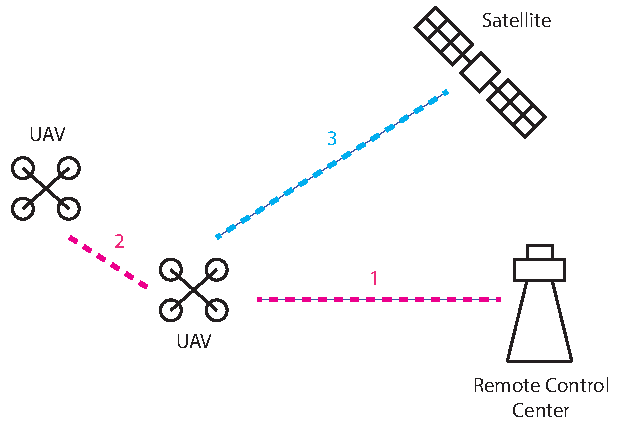
\includegraphics[width=0.5\textwidth]{chapters/se_linear/figures/qh/uav_pic.pdf}
\caption{Different communication channels that are subject to adversarial attacks: Channels 1 and 2 are vulnerable to attack in the MITM attack example (Section 5.3.1) and Channel 3 is vulnerable to attack in the GPS spoofing example (Section 5.3.2).}
\label{fig:ex_uav_pic}
\end{figure}


%%%%%%%%%%%%%%%%%%%%%%%%%%%%%%%%%%
%%%%%%%%%%%%%%%%%%%%%%%%%%%%%%%%%%

\subsection{UAV Model}

We consider a quadrotor with the following dynamics:
\begin{equation}
\begin{aligned}
x(k+1) &= A_0 x(k) + B u(k)  + k + w(k) \\
y(k) &= C x(k) + e(k) + v(k) \\
\end{aligned}
\end{equation}
where $x = [p_x, v_x, \theta_x, \dot \theta_x, p_y, v_y, \theta_y, \dot\theta_y, p_z, v_z]^T$ is the state vector. $p_x$, $p_y$ and $p_z$ represent the quadrotor's position along the $x$, $y$ and $z$ axis, respectively. $v_x$, $v_y$ and $v_z$ represent its velocities. $\theta_x$ and $\theta_y$ are the pitch and roll angles respectively, $\dot \theta_x$ and $\dot \theta_y$ are their corresponding angular velocities. %\st{represents the quadrotor's position, velocity, pitch and roll angles and angular velocities.} 
$u = [\theta_{r,x}, \theta_{r,y}, F]^T$ is the input vector: $\theta_{r,i}$ is the reference pitch or roll angle, and $F$ is the commanded thrust in the vertical direction. $y = [\tilde{p}_x, \tilde{p}_y, \tilde{p}_z]^T$ %\st{$y = [p_x, p_y, p_z]^T$}
represents compromised position measurements from the GPS under attack signal $e$. $w$ and $v$ represent process and measurement noise respectively. $k$ is a constant vector which represents gravitational effects, and can be dropped without loss of generality because we can always subtract it out in $u$. $A_\theta^{i,j}$ refers to the $ij$-th entry of the subsystem matrix of the discretized rotational dynamics $A_\theta$, and $B_\theta^i$ refers to the $i$-th entry of the input-to-state map $B_\theta$ for the discretized rotational dynamics. $T_s$ is the discrete time step, $g$ is the gravitational acceleration, $m$ is the mass of the quadrotor and $K_T$ is a thrust coefficient. Further details about this model and its derivation can be found in \cite{Bouffard}. Finally, the matrix $C$ depends on the particular measurements taken in each example.

\begin{figure}[t]
\center
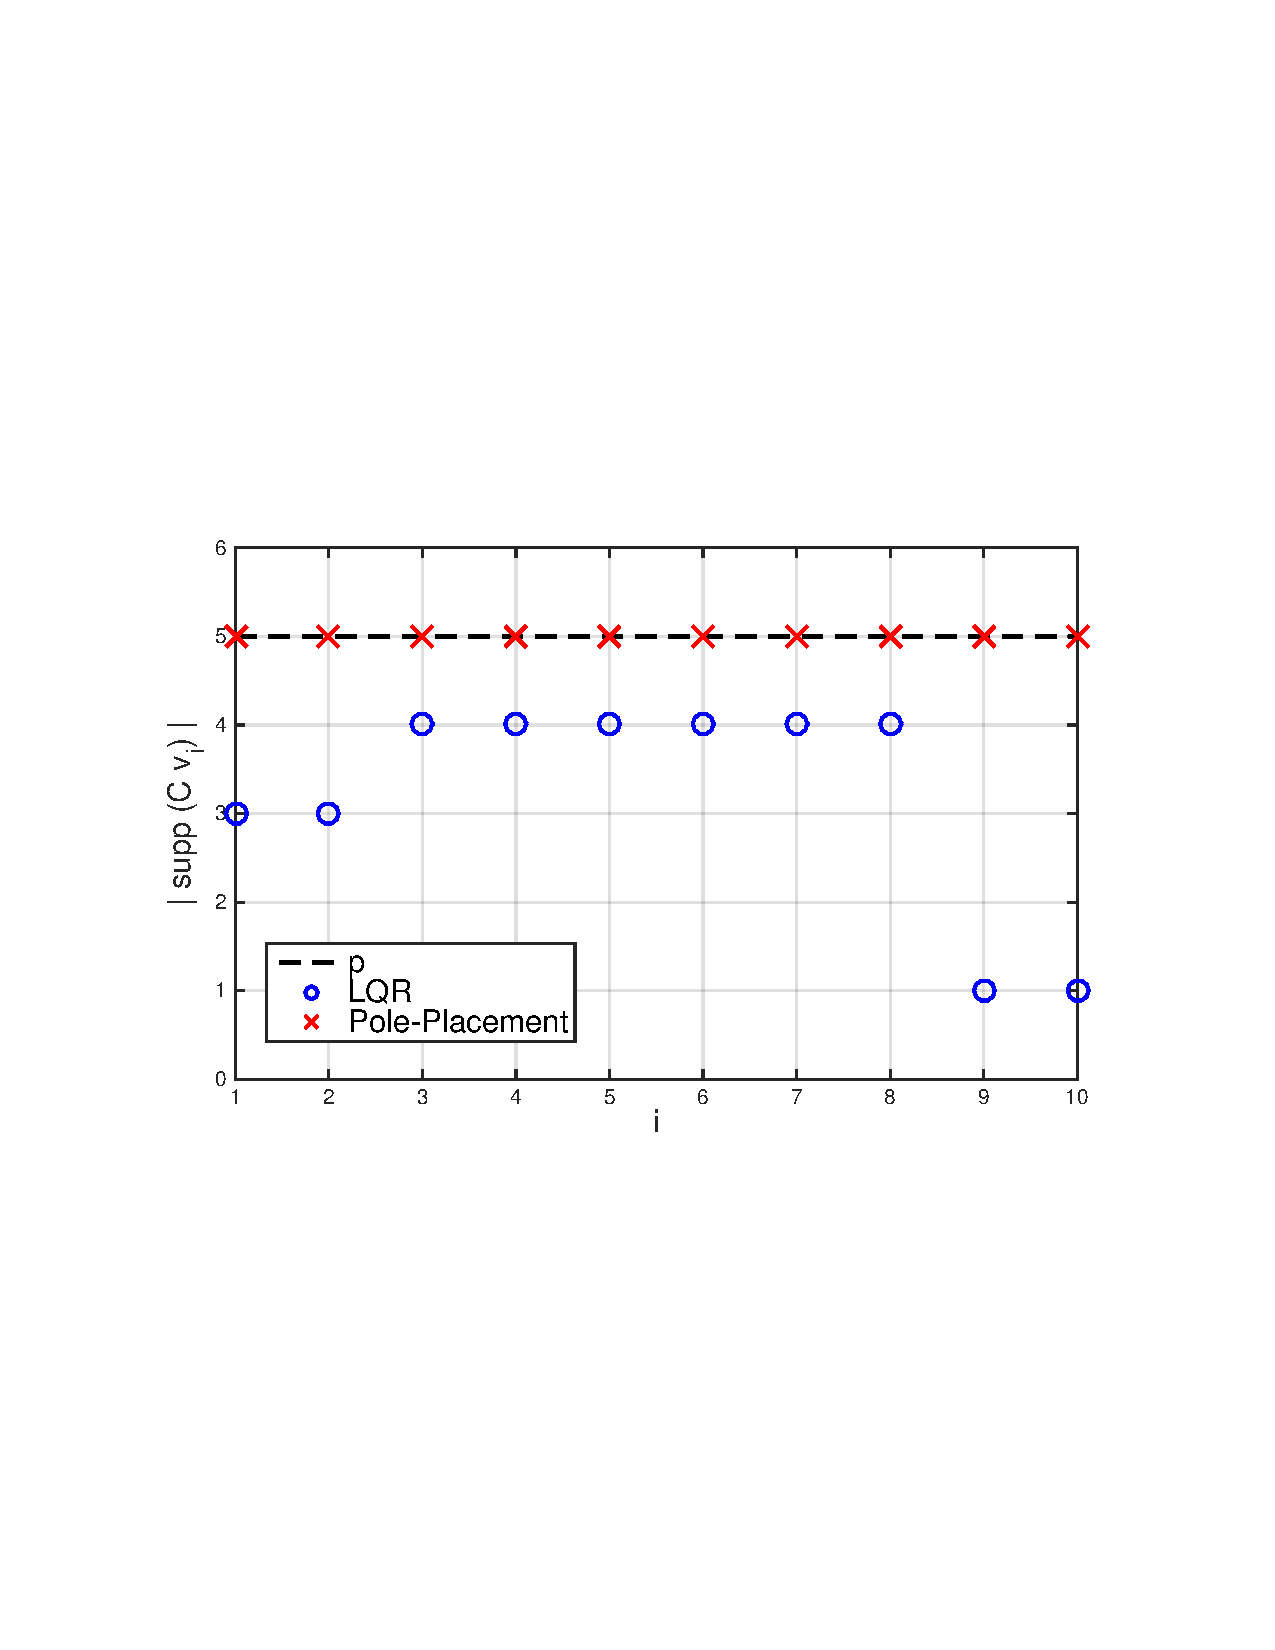
\includegraphics[width=0.6\textwidth]{chapters/se_linear/figures/supp_ev_2.pdf}
\caption{$ \lvert \textsf{supp} (C v_i) \rvert $ for all eigenvectors $v_i$ of closed-loop matrix $A$ for 2 feedback controllers: a LQR and a controller designed by pole-placement. Black dashed line is at $p = 5$, i.e., the number of measurements.}
\label{fig:ex_pole}
\end{figure}


%%%%%%%%%%%%%%%%%%%%%%%%%%%%%%%%%%
%%%%%%%%%%%%%%%%%%%%%%%%%%%%%%%%%%

\subsection{Estimator Design via Pole-Placement}

Assume that the UAV uses the state feedback control law $u(k) = G x(k)$, where $G$ is the feedback matrix which can be designed\footnote{In the GPS spoofing example, direct uncorrupted state measurements are not available. Therefore a KF is used to give estimated states which are then used for state feedback control.}. If the pair $(A_0, B)$ is controllable, then we can choose $G$ to place the closed loop poles anywhere in the complex plane. We first design a Linear Quadratic Regulator (LQR) and evaluate its secure estimation performance by checking whether the sufficient condition for $q$-attack correction  (i.e., $\lvert \textsf{supp} (C v_i) \rvert > q$ for all $i$) holds. 
Figure \ref{fig:ex_pole} shows the results for a matrix $C \in \mathbb{R}^{5\times 10}$ (i.e., 5 measurements) and observe that $\lvert \textsf{supp} (C v_i) \rvert < p = 5$ for $i=1,2,9$ and $10$. Furthermore, $\lvert \textsf{supp} (C v_i) \rvert = 1 > 0$ for $i = 9$ and $10$, therefore the resulting secure estimator can correct zero attacks!
To improve the secure estimation performance, we perturb the closed-loop poles slightly until $\lvert \textsf{supp} (C v_i) \rvert = p$ for all $i$, as shown in Figure \ref{fig:ex_pole}. Therefore the resulting secure estimator can achieve the maximum number of correctable attacks within the limits of $p$ (i.e., the number of measurements). By keeping the perturbations on the poles small, our final controller achieves both good control and estimation performances (see Figure \ref{fig:ex_pp_est}).% and \ref{fig:ex_pp_err}). 


%%%%%%%%%%%%%%%%%%%%%%%%%%%%%%%%%%
%%%%%%%%%%%%%%%%%%%%%%%%%%%%%%%%%%


\subsection{UAV under Adversarial Attack}

\subsubsection{Man-In-The-Middle (MITM) Attack in Communication with a RCC or with other UAVs} \label{sec:uav_utm}

In this section, we consider MITM attacks targeted at Channels 1 and 2 in Figure \ref{fig:ex_uav_pic}, where a malicious agent spoofs the information being sent and/or received over these channels. The goal of the RCC or other UAVs is to accurately estimate the true flight path of a target UAV from corrupted measurements. 
Note that the true path of the target UAV is unaffected by the attack.
Assume that the attacker spoofs the position measurements in order to deceive the receiver that the target UAV is deviating in the $x$-direction, i.e., she injects a continuous and increasing signal in the $x$-position measurement.
To make the estimation task even harder for the receiver, the attacker also injects a random Gaussian noise to an additional measurement, and the choice of this measurement can change at each time step. 

In this example, we first demonstrate the effectiveness of our proposed estimator design via pole-placement method by comparing the estimation performance of the estimator resulting from (1) a LQR controller and (2) a controller designed using pole-placement as described in the previous section.
%We then implement the latter feedback controller, and compare the performance of three different state estimation schemes: (1) KF only (KF), (2) secure estimator only (SE), and (3) secure estimator combined with KF (KF+SE). 
Throughout this example, $y \in \mathbb{R}^5$, measurements include the $x$, $y$ and $z$ positions and 2 additional randomly selected states. 

The left plots in Figure \ref{fig:ex_pp_est} show the true attack signal on all 5 sensors (solid lines) and the estimated attack signals (dashed lines) by the secure estimator if the feedback controller is a LQ regulator (top) or one designed via pole-placement (bottom). It is obvious that the latter estimates the attack signal much more accurately. The right plots of this figure highlights this observation by explicitly showing the estimation error of the attack signal for each measurement.

The same information is shown in Figure \ref{fig:ex_pp_err}, where each row corresponds to one sensor, and the first 3 rows are the $x$, $y$ and $z$ position measurements, respectively. This figure highlights three points: first, the attacked sensors change with time; second, the number of attacked sensors at each time $k$ is less or equal to 2; third, only position measurements are corrupted.

 
Note that the poor performance is not an inherent feature of LQR. 
Since LQR does not consider the conditions for secure estimation, there is no guarantee of good secure estimation performance. %, as shown in Figures \ref{fig:ex_n8p10} and \ref{fig:ex_n8_overall}.
On the other hand, if we satisfy the guaranteed conditions for accurate secure estimation, then we can correctly estimate the true attack signals, i.e., achieve good secure estimation performance (although we may loose some control performance).

Next, we implement feedback controller (2), i.e., one designed with pole-placement, and compare the performance of three different state estimation schemes: (a) KF only (KF), (b) secure estimator only (SE), and (c) secure estimator combined with KF (KF+SE). 
Figure \ref{fig:ex_uav_remote} shows the estimated flight paths by all three methods.
The true path of the UAV (solid blue line) starts from the position marked by the blue triangle and ends at the position marked by the blue square. KF fails to filter out the attack signal in the $x$-position measurements as the attack is highly non-Gaussian, and the estimated trajectory (dashed red line) significantly differs from the true one. On the other hand, SE correctly estimates some portions of the trajectory and the final position of the vehicle, nevertheless it produces spontaneous attacks in the $x$ direction. 
Finally the combined method KF+SE perfectly recovers the true path of the target UAV.


%%%%%%%%%%%%%%%%%%%%%%%%%%%%%%%%%%%%%%%%
\begin{figure}
\center
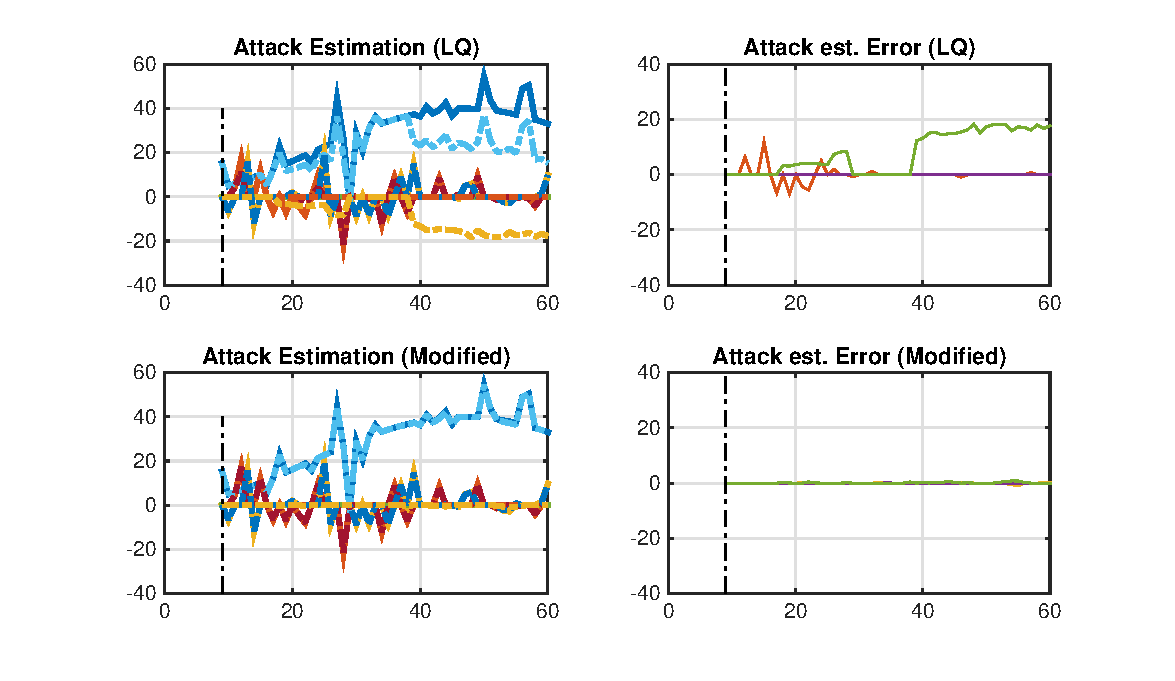
\includegraphics[width=0.8\textwidth]{chapters/se_linear/figures/qh/uav_pp_est}
\caption{True attack signal, estimated attack signal and estimation error in the attack signal of the estimator (SE) with 2 different feedback controllers: LQR, controller designed via pole-placement (PP); with 5 measurements. In the left plots, solid lines are true attack signals, dashed lines are estimated signals. The right plots show the estimation error in the attack signal.}
\label{fig:ex_pp_est}
\end{figure}
%%%%%%%%%%%%%%%%%%%%%%%%%%%%%%%%%%%%%

%%%%%%%%%%%%%%%%%%%%%%%%%%%%%%%%%%%%%
\begin{figure}
\center
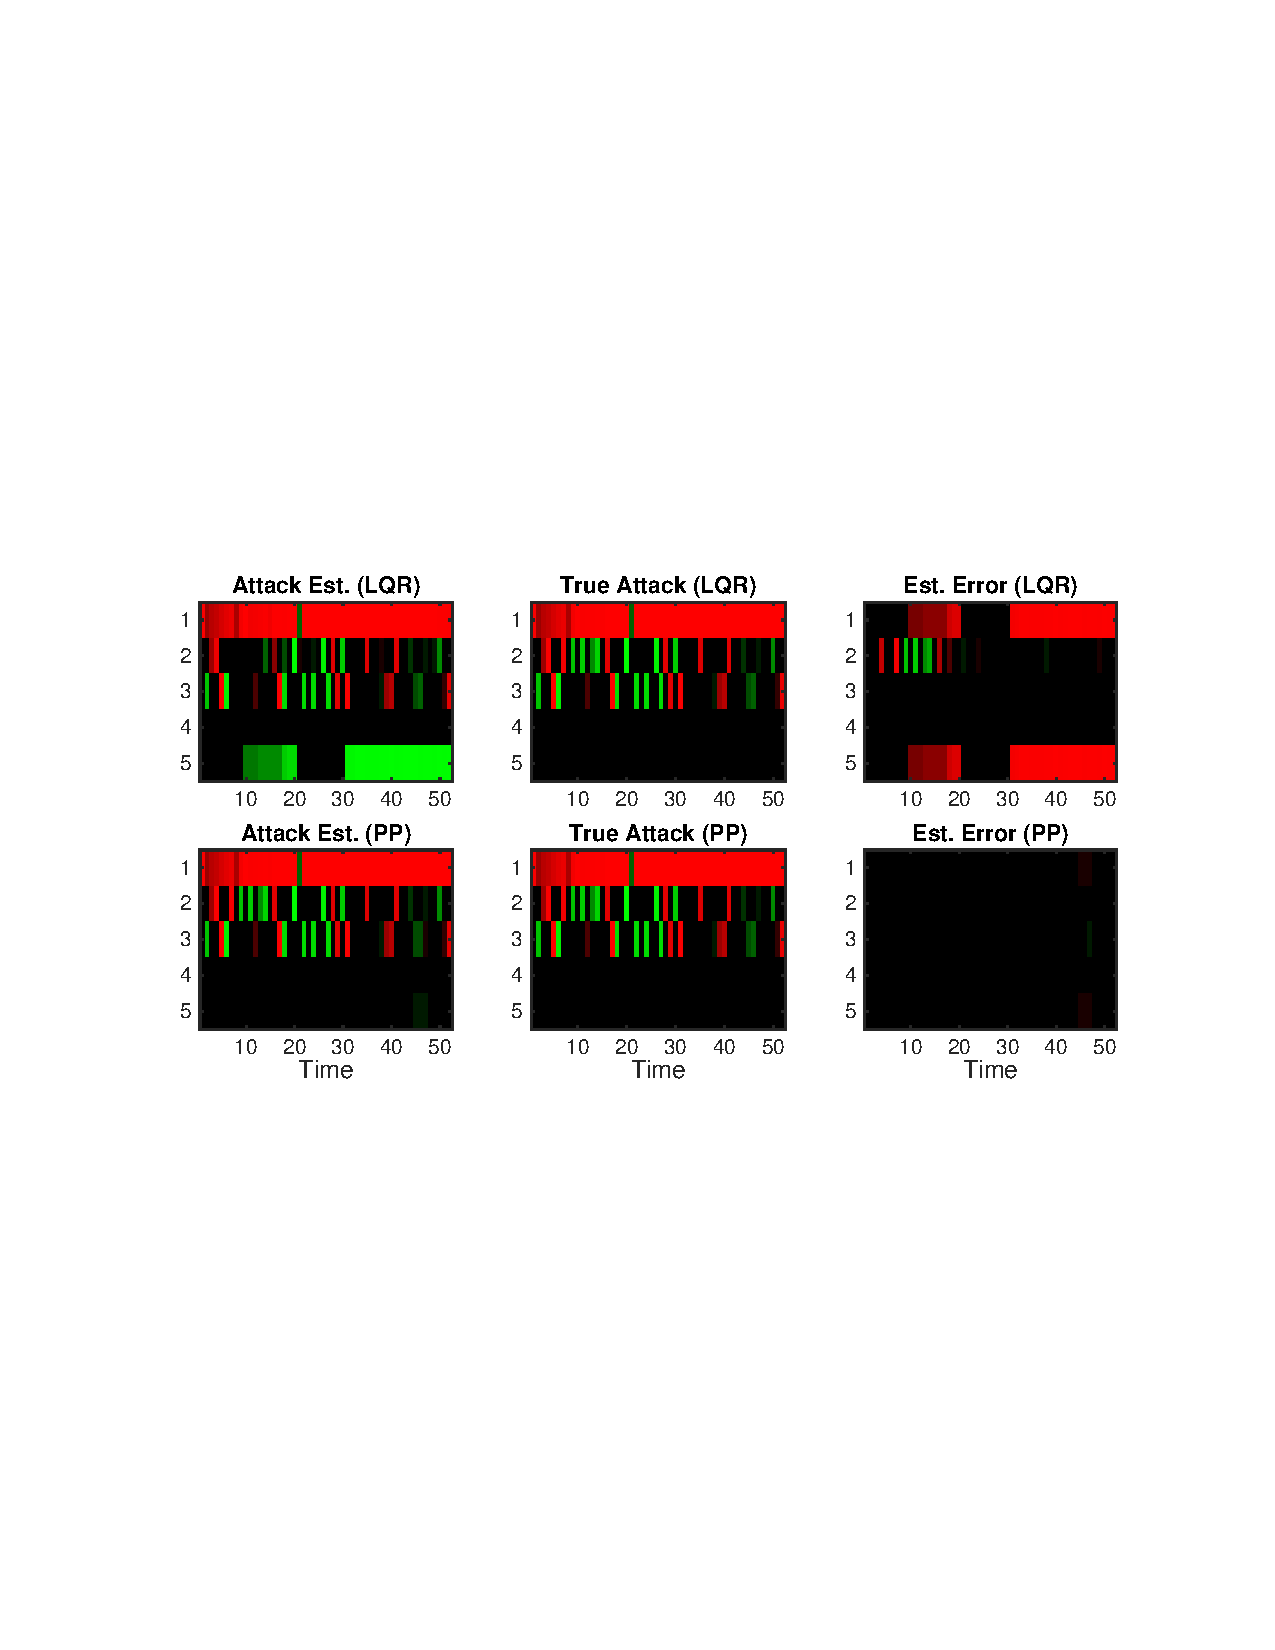
\includegraphics[width=0.8\textwidth]{chapters/se_linear/figures/qh/uav_pp_error.pdf}
\caption{Estimated attack signal, true attack signal and estimation error in the attack signal of the estimator (SE) with 2 different feedback controllers: LQR, controller designed via pole-placement (PP); with 5 measurements. Left column shows estimated attack signals. Middle column shows true attack signal. Right column shows estimation error. Each row corresponds to one type of measurement. Red pixels indicate positive values, green pixels are negative values and black indicates zero. }
%\qie{Is it necessary to include this figure? It seems repetitive from previous one.} \yh{It is repetitive from the previous one but it may help to see the structure of $E(t)$, i.e., attacked sensors change over time. Also, it would be good to understand Fig. 9}}
\label{fig:ex_pp_err}
\end{figure}
%%%%%%%%%%%%%%%%%%%%%%%%%%%%%%%%%%%%%

%%%%%%%%%%%%%%%%%%%%%%%%%%%%%%%%%%%%%
\begin{figure}
\center
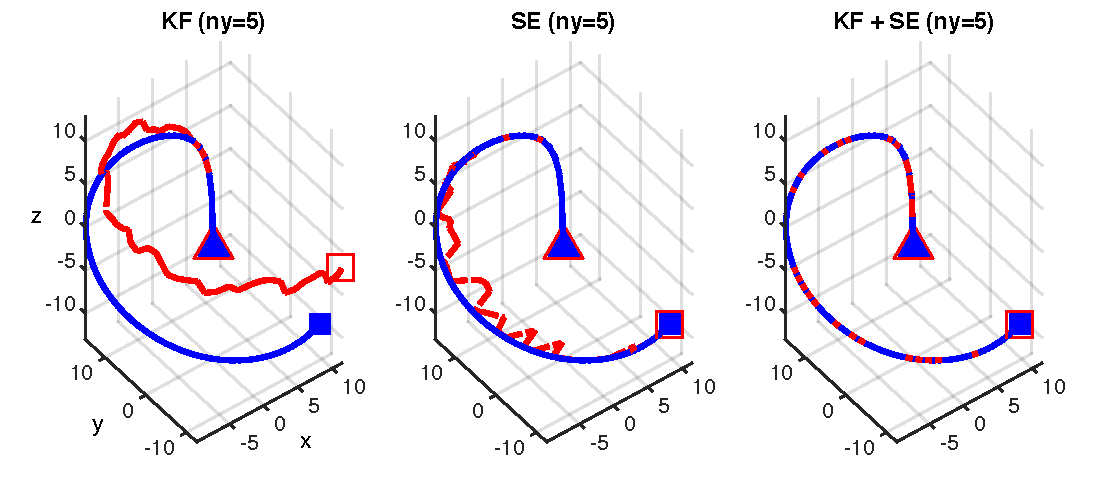
\includegraphics[width=0.9\textwidth]{chapters/se_linear/figures/qh/uav_lq_traj}
\caption{Estimated UAV trajectory by three methods under MITM attack: KF only (KF), secure estimator only (SE), secure estimator with KF (KF+SE). Solid blue lines are the true UAV trajectories. They start from the blue triangle and end at the blue square. Red dotted lines represent estimated trajectories by each method, with 5 measurements.}
\label{fig:ex_uav_remote}
\end{figure}
%%%%%%%%%%%%%%%%%%%%%%%%%%%%%%%%%%%%%

\subsubsection{GPS Spoofing}

In this section, we focus on adversarial attacks in the GPS navigation system (Channel 3 in Figure \ref{fig:ex_uav_pic}). Consider the scenario where a UAV uses a Linear Quadratic Gaussian (LQG) controller to follow a desired path, $x_r(k)$, designed by LQ control. In other words, a KF takes compromised and noisy measurements $y(k)$ and outputs a state estimate $\hat x(k)$, which is then used for state feedback control: $u(k) = G (\hat x(k) - x_r(k))$, where $G$ is the feedback matrix. Note that in the previous example (Section \ref{sec:uav_utm}), the feedback controller had access to uncorrupted state measurements $x(k)$, therefore the true path of the UAV is unaffected by attacks. On the other hand, in this example, the UAV uses estimated states $\hat x(k)$ for feedback control and path following. Hence, if measurements are corrupted and the state estimates are poor, then the UAV may not be able to follow its desired path and may deviate away from it. The goal is to correctly estimate the true states of the UAV and therefore, follow the desired path. Assume an attacker spoofs the GPS position measurements in order to deviate the UAV from its planned path. She injects a sinusoidal signal to $x$-position measurement, as well as a Gaussian noise to a randomly chosen position measurement at each time step. 

In this example, we explore the effect of the number of sensor measurements on the secure estimation performance of two schemes: (a) KF only, (b) KF+SE.
We first assume that the UAV only uses GPS for navigation, i.e., 3 positional measurements. 
Figure \ref{fig:ex_uav_traj} shows that KF completely fails to estimate the attack signal (KF, $n_y = 3$, plots in Row 1), %There are large estimation attacks in its estimated $x$- and $z$-positions, 
consequently the actual UAV trajectory (red dashed line)  deviates significantly from its desired path (solid blue line). %as shown in Figure \ref{fig:ex_uav_traj}.%, and deviations are largest along the $x$- and $z$-axis (Figure \ref{fig:ex_uav_est}).
On the other hand, Figure \ref{fig:ex_uav_traj} (KF + SE, $n_y = 3$) shows that KF+SE's estimated attack signals are significantly more accurate with only a small estimation error in the $x$-position (plots in Row 2). 
Therefore the UAV can follow its planned path much more closely. % (Figures \ref{fig:ex_uav_traj}).%  and \ref{fig:ex_uav_est}).
Recall from Proposition \ref{prop:maximum} that the maximum number of correctable attacks for a system with $p$ measurements is $\lceil p/2-1 \rceil$, which equals 1 in this case. There are at most 2 attacked sensors at any time $k$ in this example, which exceeds the above limit. This explains the estimation error in the $x$-position. Despite this small estimation error, the combined scheme KF+SE still outperforms the KF on its own.

We now show the effect of increasing the number of measurements ($n_y$, or equivalently $p$) through sensor fusion, on the estimation performance and consequently, the UAV's path following performance. Autonomous UAVs often use IMUs in addition to GPS for navigation, the former provides additional measurements such as the UAV's velocities, pitch and roll angles. Figure \ref{fig:ex_uav_traj} shows that increasing the number of measurements has no effect on the KF's estimation accuracy (compare plots in Rows 1, 3 and 5). 
Even when 8 measurements are used the UAV equipped with a KF still fails to follow the desired path. %(Figures \ref{fig:ex_uav_traj}).% and \ref{fig:ex_uav_est}). 
On the other hand, increasing the number of measurements improves the estimation performance of the secure estimator (SE) and consequently the performance of the combined scheme KF+SE. %(compare plots in Rows 2, 4 and 6 in Figure  \ref{fig:ex_uav_error}). 
Figure \ref{fig:ex_uav_traj} shows that when 5 and 8 measurements are used, the UAV can follow its original planned
path perfectly (KF + SE $n_y = 5$ and KF + SE $n_y = 8$).
%Observe that for both 3 and 5 measurements, the combined scheme KF+SE perfectly estimates the attack signals and therefore, can completely subtract them out from the corrupted measurements. As a result, the UAV can follow its original planned path perfectly (KF + SE $n_y=5$, KF + SE $n_y=8$ in Figures \ref{fig:ex_uav_traj}).% and \ref{fig:ex_uav_est}).


%%%%%%%%%%%%%%%%%%%%%%%%%%%%%%%%%%%%%
%%%%%%%%%%%%%%%%%%%%%%%%%%%%%%%%%%%%%
%%%%%%%%%%%%%%%%%%%%%%%%%%%%%%%%%%%%%

\section{Conclusion}
In this chapter, we consider the problem of secure estimation for CPS under adversarial attacks. Unlike \cite{Fawzi:2014} where the attacked sensors are assumed to be fixed, we allow the set of attacked sensors to change over time, and propose a computationally efficient secure estimator for the latter scenario that works for arbitrary and unbounded attacks. In addition, we propose to combine the secure estimator with a KF for improved practical performance. We demonstrate through numerical examples, that our proposed secure estimator based KF outperforms standard KF. Furthermore, we illustrate practical applications of secure estimation in UAVs under adversarial cyber attacks. This is important not only for today's aviation system but also UAV delivery systems in the near future. 


%%%%%%%%%%%%%%%%%%%%%%%%%%%%%%%%%%%%%%
%\begin{figure}
%\center
%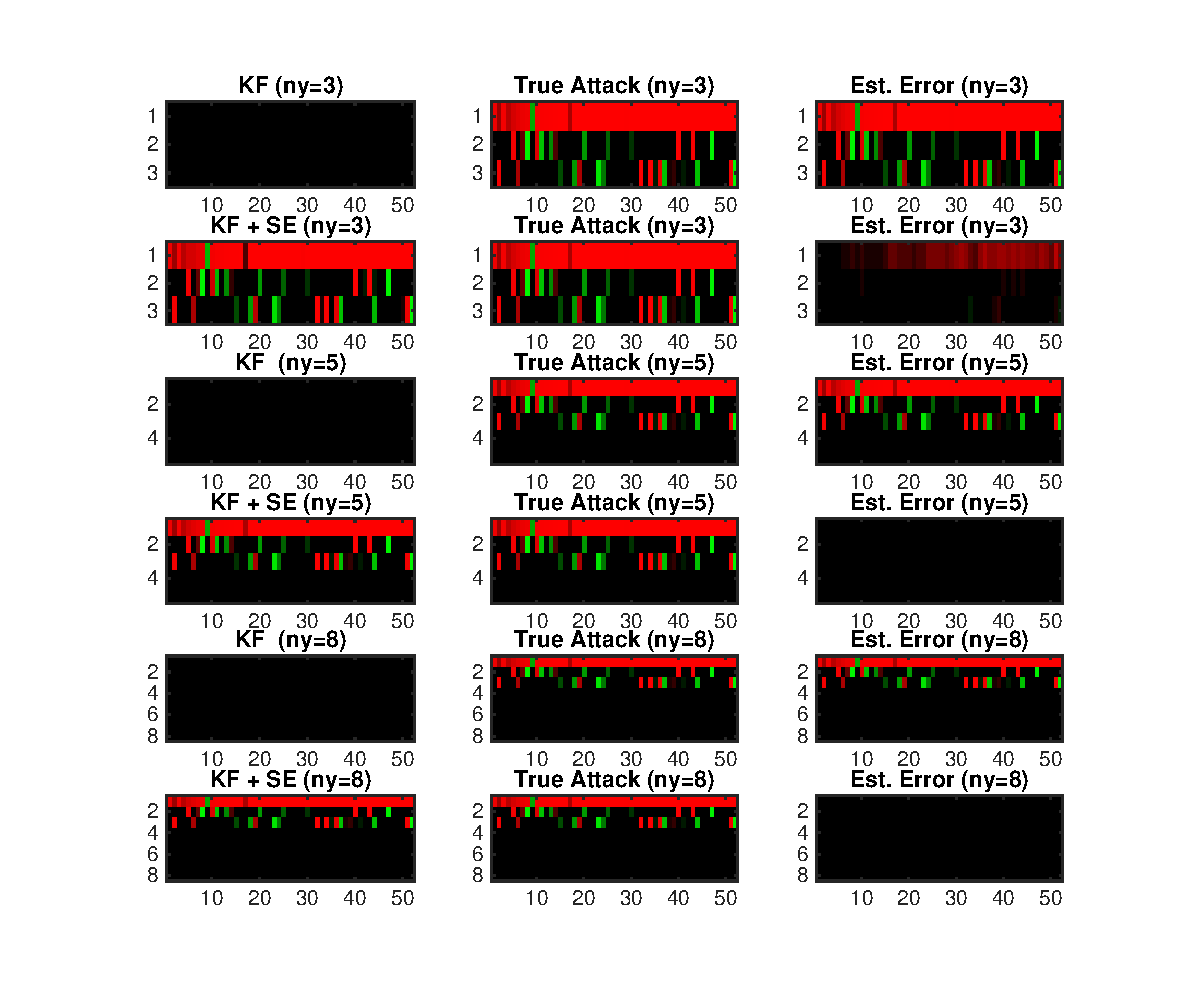
\includegraphics[width=0.9\textwidth]{chapters/se_linear/figures/qh/uav_lqg_error}
%\caption{Estimated attack signal, true attack signal and estimation error in different cases: KF and KF+SE, each using 3, 5 and 8 different measurements. Left column shows estimated attack signals. Middle column shows true attack signal. Right column shows estimation error. Each row corresponds to one sensor measurement and the first three rows in each plot are the $x$, $y$ and $z$ position measurements, respectively. Red pixels indicate positive values, green pixels are negative values and black indicates zero.}
%\label{fig:ex_uav_error}
%\end{figure}
%%%%%%%%%%%%%%%%%%%%%%%%%%%%%%%%%%%%%
\begin{figure}
\center
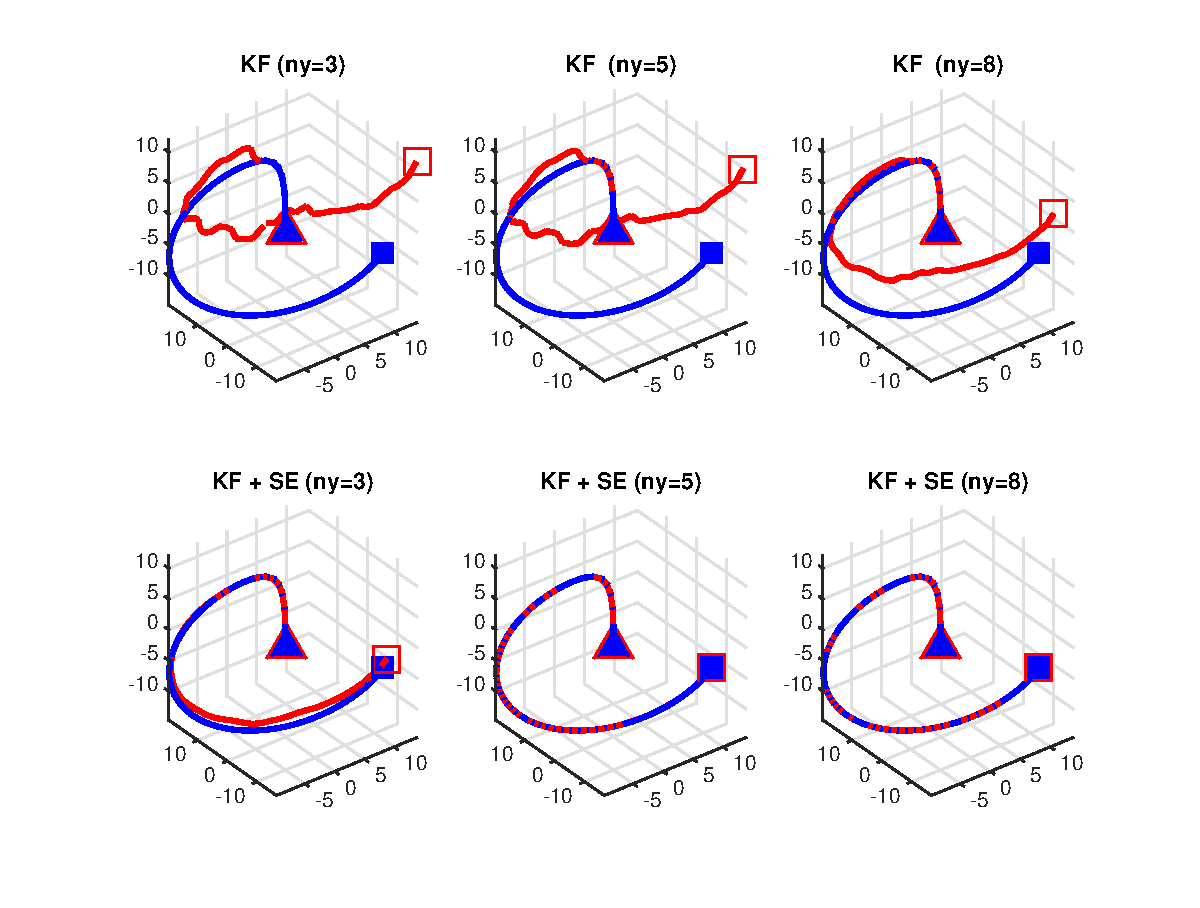
\includegraphics[width=\textwidth]{chapters/se_linear/figures/qh/uav_lqg_traj}
\caption{Desired and actual UAV trajectory in different cases: KF and KF+SE, each using 3, 5 and 8 different measurements. Blue solid lines are the desired trajectory. Red dash lines are the actual UAV trajectory under adversarial attack.}
\label{fig:ex_uav_traj}
\end{figure}
%%%%%%%%%%%%%%%%%%%%%%%%%%%%%%%%%%%%%
%\begin{figure}
%\center
%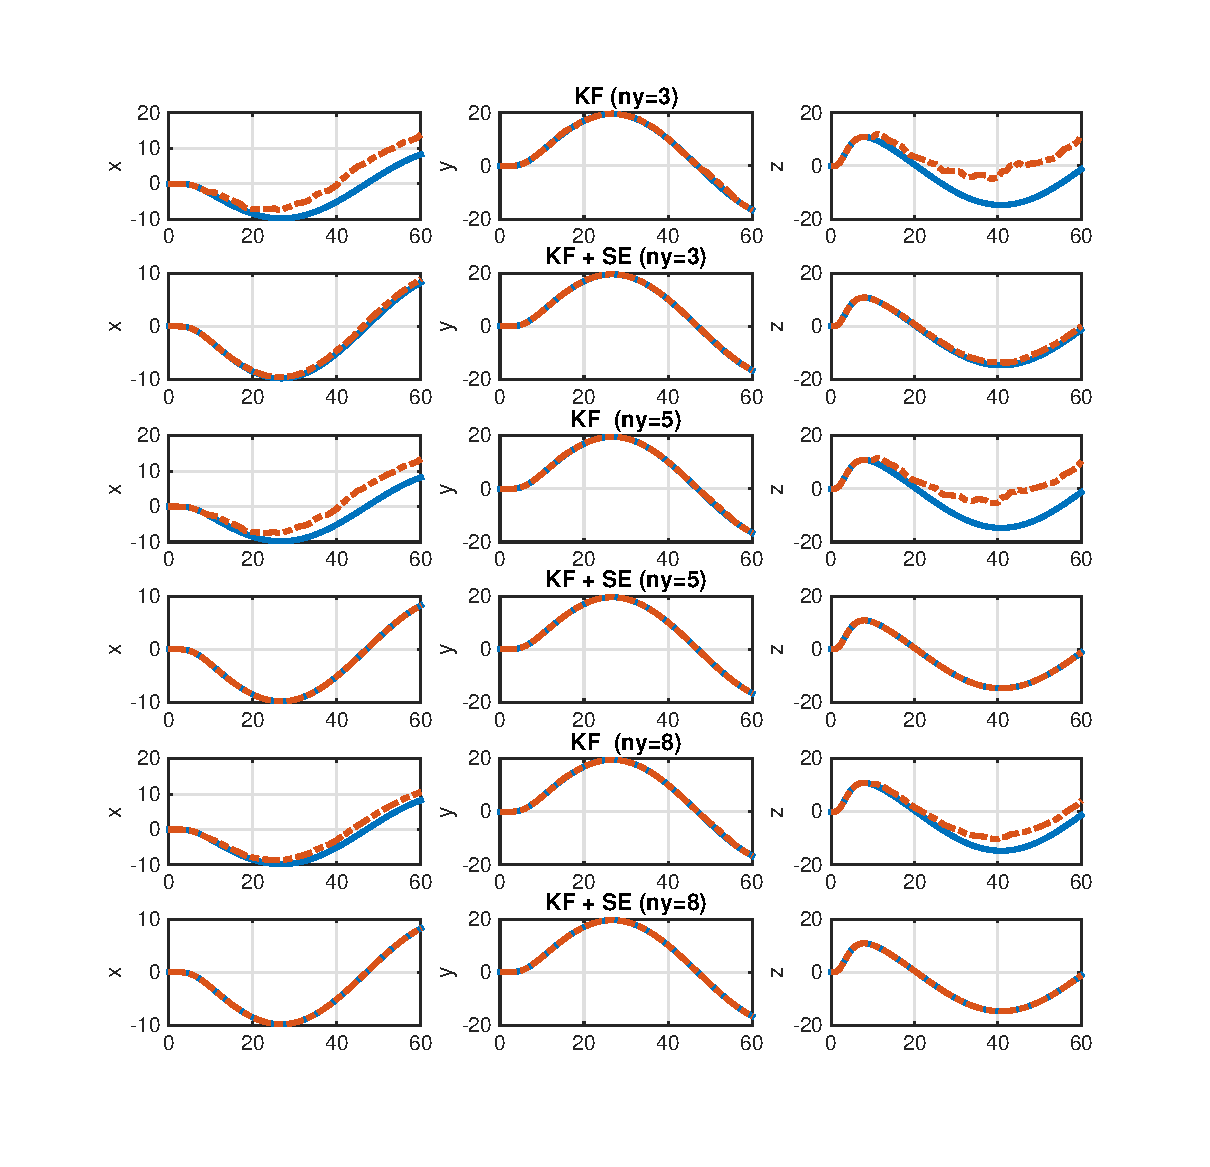
\includegraphics[width=0.9\textwidth]{chapters/se_linear/figures/qh/uav_lqg_est}
%\caption{Desired and actual UAV trajectory in different cases: KF and KF+SE, each using 3, 5 and 8 different measurements. Blue solid lines are the desired $x$, $y$ and $z$ trajectories. Red dashed lines are the actual UAV trajectories under adversarial attack.}
%%\qie{Same for this figure} \yh{What does it mean?}}
%\label{fig:ex_uav_est}
%\end{figure}


                                 

\end{document}